\section{Présentation}
Une application de démonstration a été développée.\\
Elle se trouve dans le répertoire app/SFML de la racine du projet. Il s'agit gobalement de la même simulation que celle présente dans le leçon 1. Seuls les paramètres changent, et surtout, une interface graphique basique est ajoutée afin de visualiser le processus d'affectation en temps réel.\\\\

La bibliothèque multimédia utilisée est la SFML, qui est donc requise comme dépendance pour compiler l'application. Pour compiler et utiliser l'application, reportez-vous à la section Guide utilisateur.\\\\

La encore, aucun obstacle ne se trouve sur le monde, et il n'existe pas de frontière à l'espace. Il est modélisé à l'écran par un rectangle. Les emplacements de travail sont représentés par des carrés rouges et les carrés bleus représentent les resources.\\
En haut à gauche un compte indique la valeur de la tâche définie. Une contrainte est définie sur cette tâche : elle doit être supérieure à 5000.\\\\

L'affichage et la gestion des commandes est gérée par une seule fonction qui est ajouté au contrôleur principal du framework et a un taux de rafraichissement identique à celui de l'environnement.\\
Pour faire l'affichage, 3 classes sont partiellement wrappées : environnement, resource et taskspot.

\section{Captures d'écran}

\begin{figure}[!h]\centering
    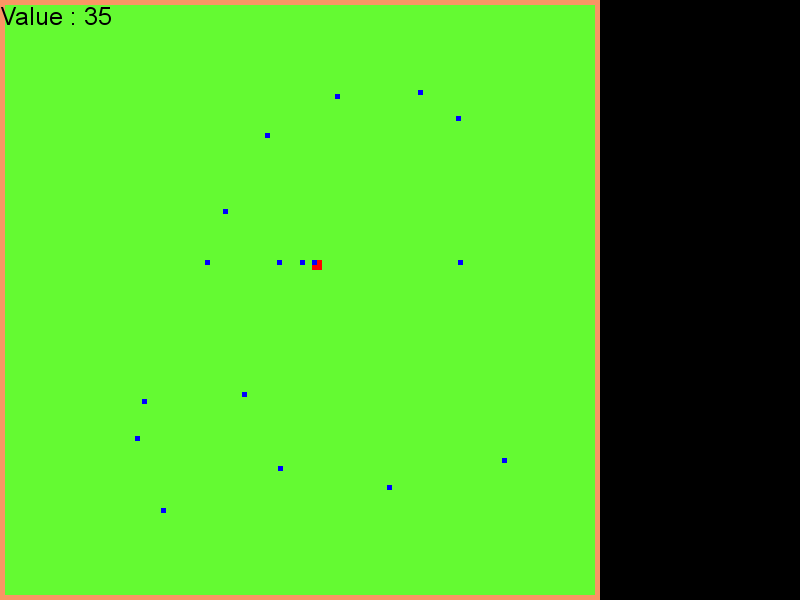
\includegraphics[scale=0.5]{screens/1.png}
\end{figure}

\begin{figure}[!h]\centering
    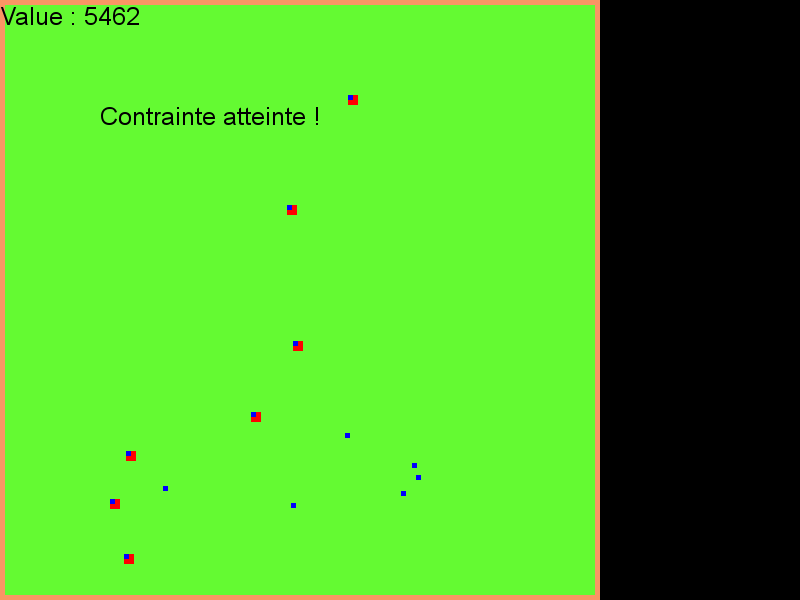
\includegraphics[scale=0.5]{screens/2.png}
\end{figure}
